% 第6章 本研究の詳細
\newpage
\renewcommand{\baselinestretch}{1.5}
\section{本研究の詳細}
\renewcommand{\baselinestretch}{1}

\par デザイナーやネットユーザーが検証するウェブページのURLおよびページのレイアウトタイプを入力すると該当ページの顕著性マップとページの構造を組み合わせることにより顕著度が高い領域を要素単位で分析して顕著領域マップを出力する手法を提案する。また、一般ユーザー向けに特に顕著度が高い領域を纏めて描写した集約図を出力する手法を提案する。本手法のモデルアーキテクチャを図\ref{fig_ourmodel}に示す。

\begin{figure}[H]
    \centering
    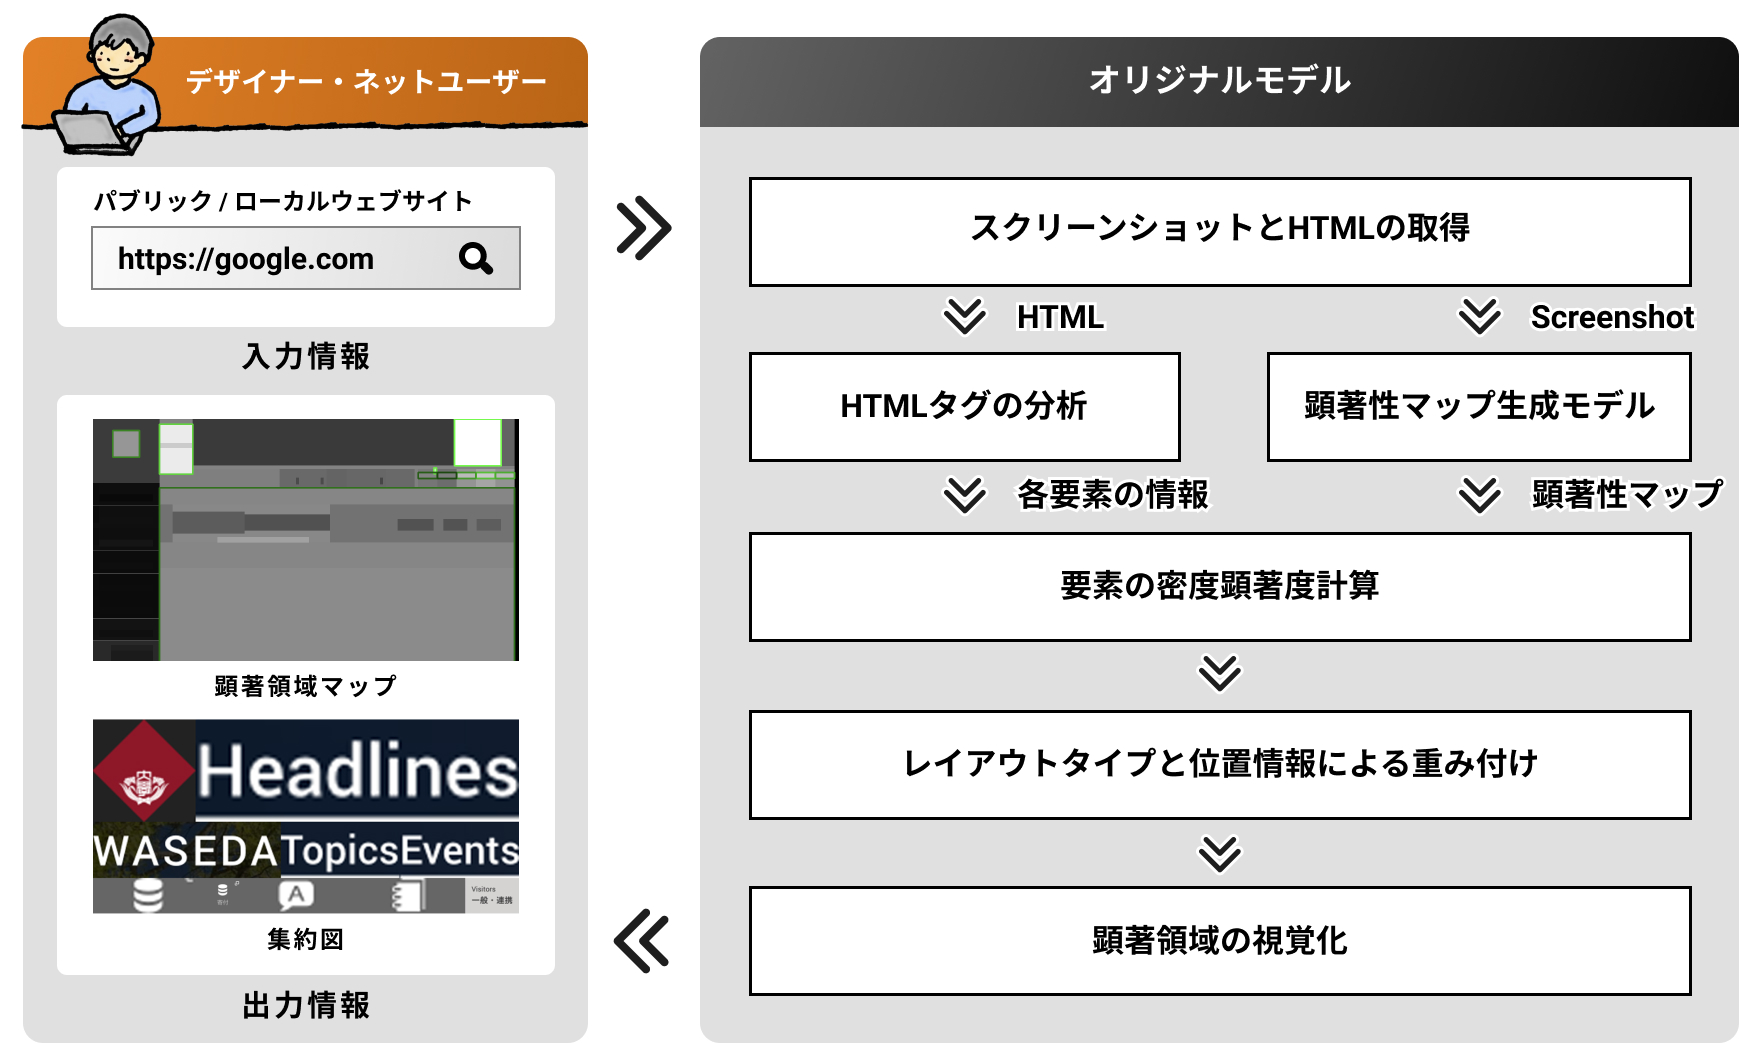
\includegraphics[width=9cm]{figures/model.jpg}
    \caption{モデルアーキテクチャ}
    \label{fig_ourmodel}
\end{figure}

\par 本手法の手順は大きく分けて以下の4つである。
\par(1) HTMLの取得と顕著性マップの生成
\par(2) HTMLの解析によるタグの分析と位置情報の取得
\par(3) レイアウトタイプを考慮した要素の顕著度計算
\par(4) 顕著領域の視覚化\\

\par なお、本研究ではサーバーサイドのプログラムを使用することで外部サーバーにアクセスしてウェブサイト上から必要な情報を取得するウェブスクレイピング技術としてウェブアプリケーションの自動テストツールであるSelenium WebDriver\cite{selenium}や取得したHTMLからタグや必要な情報を取得するPython用のライブラリであるBeautiful Soup\cite{beautifulsoup}を使用するが別のスクレイピング技術を使用しても実装は可能である。また、スクリーンショットを取得するウェブブラウザとしてFirefoxを使用するがChromeなど別のブラウザでも実装可能である。

\subsection{HTMLの取得と顕著性マップの生成}\label{subsec:system01}
\par 本システムではまず、入力されたURL情報を元にウェブスクレイピング技術を用いてスクリーンショットとHTMLを取得する。また、取得したスクリーンショットを用いて顕著性マップを生成する。デザイナーが開発段階で簡単に使用可能な様に入力するURLは、ネットワーク上に存在するウェブページだけでなくローカル環境のURLにも対応させている。HTMLの取得と顕著性マップの生成の流れを図\ref{fig_system01}に示す。

\begin{figure}[H]
    \centering
    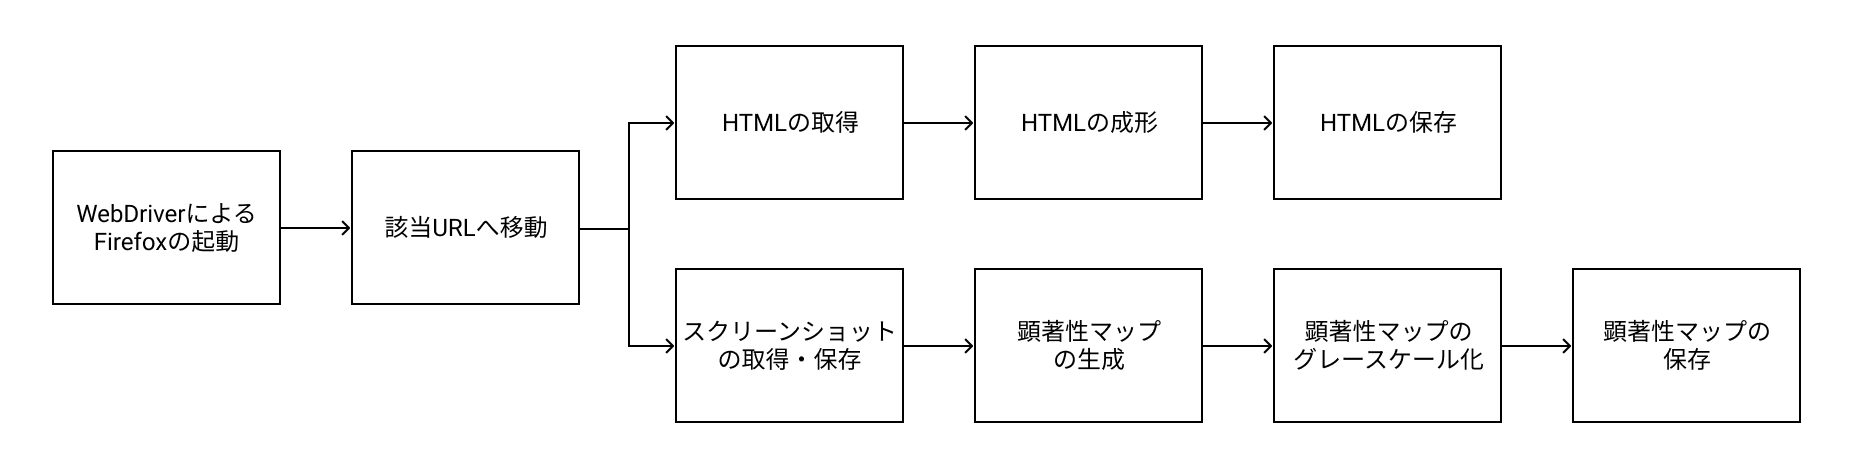
\includegraphics[width=12cm]{figures/06_process01.jpg}
    \caption{HTMLの取得と顕著性マップの生成の流れ}
    \label{fig_system01}
\end{figure}

\par まず始めに、Selenium WebDriverを用いてFirefoxを起動し、ブラウザのウィンドウサイズを一般的なパソコンで閲覧する条件に近い横1280px縦900pxに設定する。次に入力されたURLにアクセスを行い、ウェブページの読み込みが完了したらHTMLの取得を行う。取得したHTMLはインデントなどが乱れた状態である為、Selenium WebDriverと同じくウェブスクレイピング技術のライブラリであるBeautiful Soup\cite{beautifulsoup}を使用して扱いやすい状態に整形を行った後に保存する。

\par 次にウェブページのスクリーンショットを取得する。取得するスクリーンショットは、重要度が高いコンテンツはウェブページの最上部に存在する可能性が高いという考えから、ウェブページにアクセスした時点で閲覧可能な最上部の横1280px縦900pxとした。さらに、取得したスクリーンショットから顕著性マップを生成する。顕著性マップの生成には人間の目の視覚認識と同様に色・輝度・方向のそれぞれの視覚特徴を抽出した後に重み付けして足し合わせることにより顕著性マップを生成する最もベーシックなモデルのItti-Kochらの顕著性マップ生成モデルをベースに使用した。顕著性マップ生成モデルには深層学習を使用した精度の高いモデルまで幅広く存在しているが、特にバイアスを考慮しておらず扱いやすいモデルを使用することにした。
\par ここで顕著性マップ生成モデルにより出力される顕著性マップはRGBの3色チャンネルで出力されるが、計算処理を行いやすいように単色チャンネルで表されるグレースケール画像に変換して保存する。図\ref{fig_06_example_saliencymap}に早稲田大学ウェブサイトトップページ(2021年1月時点)\cite{waseda_top}のスクリーンショットを入力した時に生成される取得されるグレースケール顕著性マップの例を示す。

\begin{figure}[H]
  \centering
  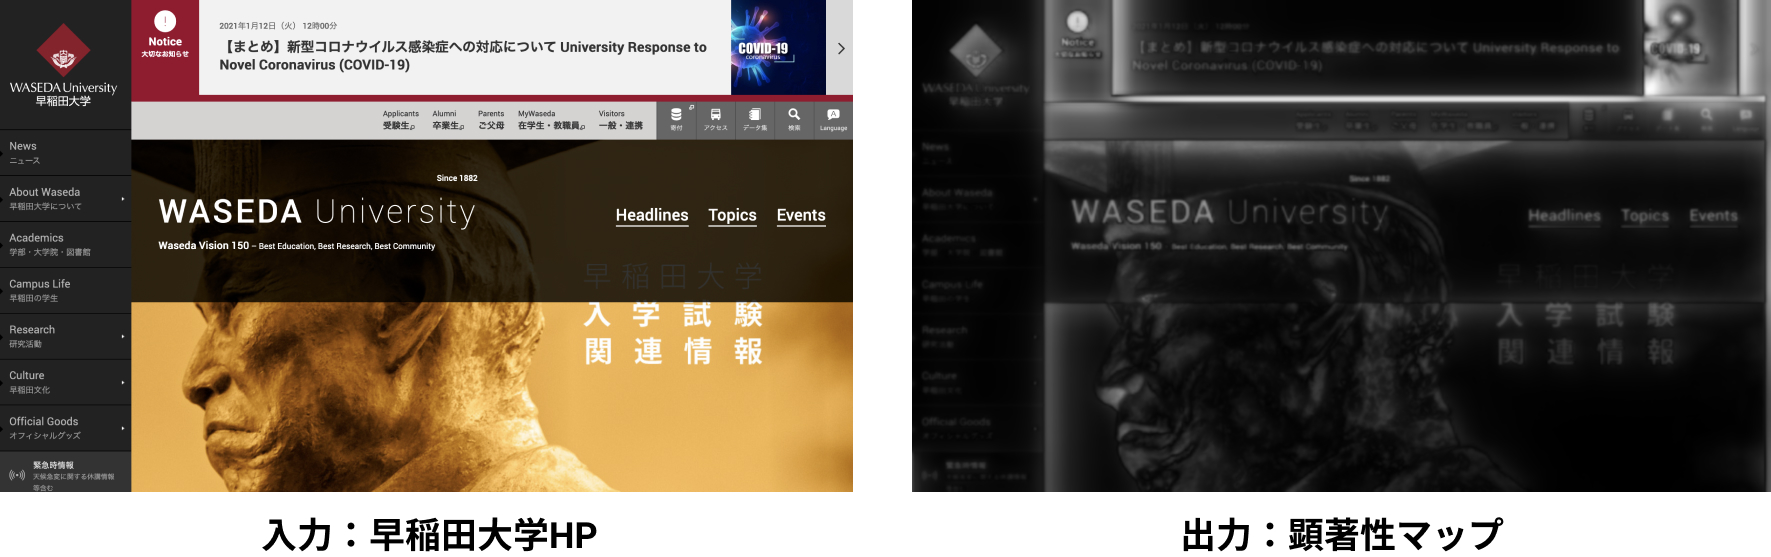
\includegraphics[width=12cm]{figures/06_ex-saliencymap}
  \caption{出力されるウェブページの顕著性マップの例}
  \label{fig_06_example_saliencymap}
\end{figure}


\subsection{HTMLの解析によるタグの分析と位置情報の取得}\label{subsec:system02}
\par ここでは第\ref{subsec:system01}節で取得したHTMLの解析を行いウェブページ上の要素の位置情報とそのサイズを取得する。HTMLの解析によるタグの分析と位置の取得の流れを図\ref{fig_system02}に示す。

\begin{figure}[H]
    \centering
    
\includegraphics[width=12cm]{figures/06_process02.jpg}
    \caption{HTMLの解析によるタグの分析と位置の取得の流れ}
    \label{fig_system02}
\end{figure}

\par まず始めに第\ref{subsec:system01}節で取得したHTMLの分析を行い、Selenium WebDriverで表\ref{table:gettaglist}に示す7個のタグ要素のidまたはclass名と左上の頂点の座標と縦と横のサイズを取得してそれらの情報をデータベースに記録する。各要素の座標の取得方法については、ウェブブラウザの表示領域の左上を基準点(0,0)として基準点からの距離を要素の座標とした。また、時間短縮とエラーを防ぐために取得したスクリーンショット領域内に表示されている要素のみを取得する。早稲田大学ウェブサイトトップページ(2021年1月時点)\cite{waseda_top}および、Yahoo! JAPANトップページ(2021年1月時点)\cite{yahoo}のウェブページの要素情報を取得して、直線で各要素を囲んだ例を図\ref{fig_06_ex-lineview}に示す。表示領域の指定要素のサイズと位置を取得している事が確認できる。

\begin{table}[h]
    \caption{位置情報とサイズを取得するタグの一覧}
    \label{table:gettaglist}
    \centering
     \begin{tabular}{clll}
      \hline
      要素名 & タグ & 意味 \\
      \hline \hline
      ブロック要素 & \textless div\textgreater & ブロック要素を表す \\
      見出し1 & \textless h1\textgreater & 文書中の見出しを示す為の要素で最も重要 \\
      見出し2 & \textless h2\textgreater & 文書中の見出しを示す為の要素で2番目に重要 \\
      見出し3 & \textless h3\textgreater & 文書中の見出しを示す為の要素で3番目に重要 \\
      リンク & \textless a\textgreater & リンクを示す \\
      インライン要素 & \textless span\textgreater & インライン要素を示し、重要な要素が多い \\
      段落 & \textless p\textgreater & テキスト要素を表す \\
      入力欄 & \textless input\textgreater & フォームなどの入力要素を表す \\
      イメージ & \textless img\textgreater & 画像要素を表す \\
      \hline
    \end{tabular}
\end{table}

\begin{figure}[H]
  \centering
  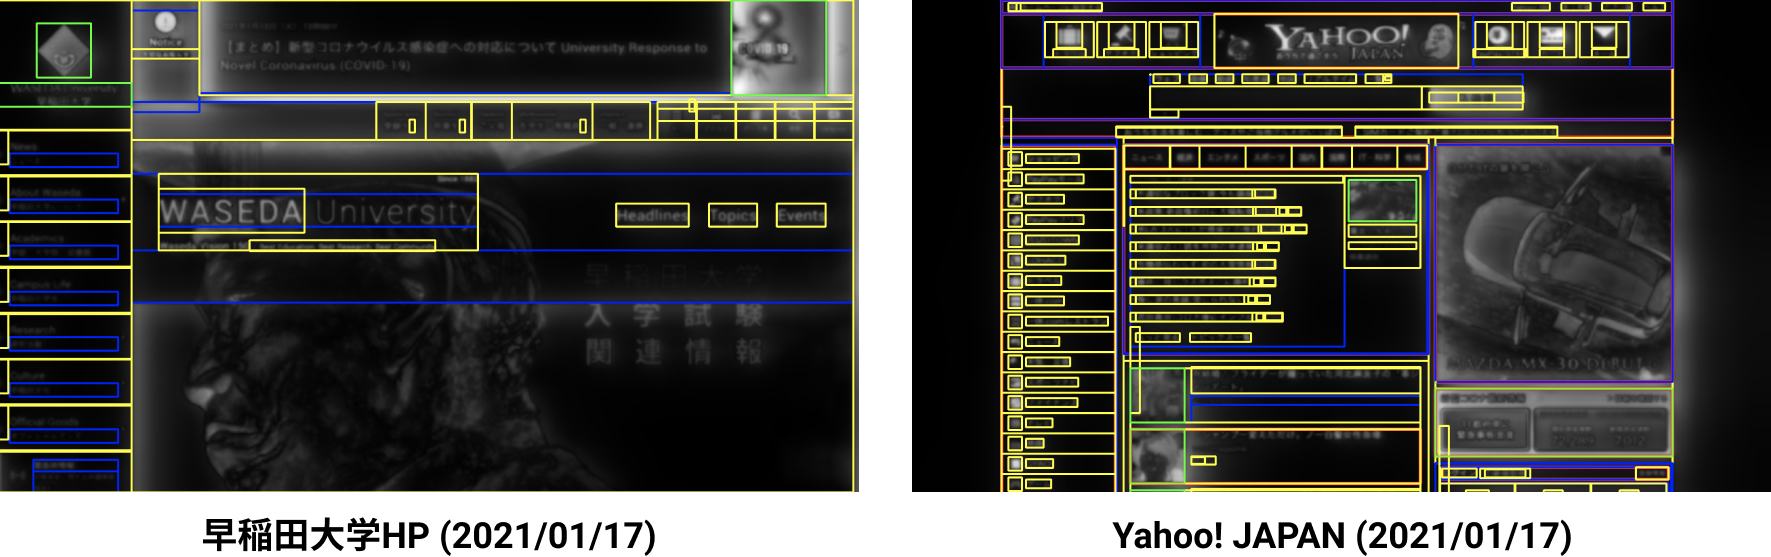
\includegraphics[width=12cm]{figures/06_ex-lineview.jpg}
  \caption{ウェブページの要素の取得の様子}
  \label{fig_06_ex-lineview}
\end{figure}

\subsection{レイアウトタイプを考慮した要素の顕著度計算}\label{subsec:system03}
\par ここでは第\ref{subsec:system01}節で生成した顕著性マップと第\ref{subsec:system02}節で取得した各要素の位置情報とサイズを組み合わせて各要素の顕著度を計算する。レイアウトタイプを考慮した要素内顕著度の計算の流れを図\ref{fig_system03}に示す。

\begin{figure}[H]
    \centering
    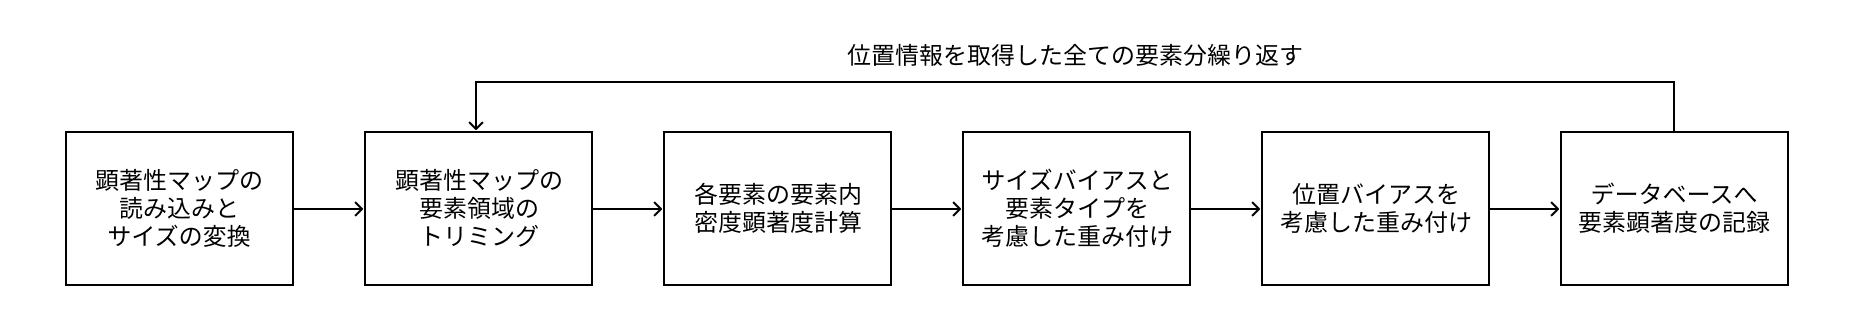
\includegraphics[width=12cm]{figures/06_process03.jpg}
    \caption{顕著度の計算の流れ}
    \label{fig_system03}
\end{figure}

\par まず始めに第\ref{subsec:system01}節で作成した顕著性マップを読み込む。使用端末により異なるが最近のパソコンは画面の高画質化が進み、AppleのRetinaディスプレイなどの高精細ディスプレイでは複数のピクセルで1つのドットを表しており倍近い解像度でスクリーンショットが保存されている。その為、単純に顕著性マップを読み込み要素の位置情報と照らし合わせるとズレが生じる。この問題を解決する為に読み込んだ顕著性マップを圧縮して実際にウェブブラウザ上で取得した位置情報と同じサイズに合わせる必要がある。

\par 次に第\ref{subsec:system02}節で取得した各要素ごとの顕著度を計算するために顕著性マップの該当要素の領域をトリミングする。また、トリミングした領域のピクセルレベルでの顕著度の積分を要素面積の平均顕著度で割る事で要素の密度顕著度を計算する。具体的な計算方法をアルゴリズム\ref{alg:element_saliency}に示す。従来は要素内部のピクセルレベルの顕著度の平均を顕著度としていたが、要素のピクセルレベルでの密度顕著度を計算したことで、小さな要素から大きい要素までバランスよく顕著度を評価する事が可能である。

\par しかしながらアイコンなどの極端に小さい要素の顕著度が過剰に高く評価されてしまうなどの問題が生じた。またウェブページの左上から中央にかけての領域に視線が集まりやすいf-biasなどのウェブページ固有の現象なども存在する。それらの問題を解決するために、本システムでは要素のサイズと位置情報によるレイアウトを考慮した顕著度の重み付けを行う事でより正確に顕著度を判定出来るように工夫した。

\begin{algorithm}[H]
  \small
  \caption{要素の顕著度計算手法}
  \label{alg:element_saliency}
  \begin{algorithmic}
  \Function{get\_element\_salient\_level}{start\_x, start\_y, end\_x, end\_y}
  \If{(end\_x - start\_x) $>$ 0 and (end\_y - start\_y) $>$ 0}
    \State cliped = Element.canvas.cv2[start\_y:end\_y, start\_x:end\_x] //要素をトリミング
    \State element\_occupancy = $\frac{(end\_x - start\_x) \times (end\_y - start\_y)}{width * height}$ //要素の占有率を計算
    \State salient\_level = $\frac{get\_element\_total\_saliency(cliped)}{get\_total\_saliency() \times element\_occupancy}$ //要素の顕著度を計算
    \State \Return salient\_level
  \Else
    \State \Return 0
  \EndIf
  \EndFunction
  \State
  \Function{get\_total\_saliency}{}
    \State clipped = Element.canvas.cv2[0:height, 0:width] //ウェブページ全体
    \State total\_saliency\_per\_row = np.sum(clipped, axis=0) //行の色の合計を取得
    \State total\_saliency = np.sum(total\_saliency\_per\_row, axis=0) //列の色の合計を取得
    \State \Return np.uint8(total\_saliency)
  \EndFunction
  \State
  \Function{get\_element\_total\_saliency}{clipped}
    \State total\_saliency\_per\_row = np.sum(clipped, axis=0) //行の色の合計を取得
    \State total\_saliency = np.sum(total\_saliency\_per\_row, axis=0) //列の色の合計を取得
    \State \Return np.uint8(total\_saliency)
  \EndFunction
  \end{algorithmic}
\end{algorithm}

\subsubsection{要素のサイズと要素タイプによる重み付け}\label{subsec:system03-1}
\par 先ほど述べた通り、アイコンなどの極端に小さい要素の顕著度が極端に高く計算される傾向があることが判明した為、要素の大きさによる重み付けを行うことで顕著度の偏りをなくす。ウェブページに存在するアイコンには様々なサイズのものが存在する。また画像要素だけでなく、CSSで描写されたアイコンやdiv要素にbackgroundプロパティで指定されたものなど要素のタイプも様々である。そこで本システムでは一般的にアイコンと呼ばれるサイズ以下の要素の重みを変更して適切な顕著度を計算する事にした。

\par 我々が日常でよく閲覧するアイコンとしてWindowsやMacやIOSなどのOS標準のアイコンが存在する。MicrosoftによるとWindowsではダイアログボックスやエラーページなどに32px$\times$32pxのアイコンが標準サイズとして使用されている\cite{windowsicon}。また、iPhoneなどのIOSやMacには64px$\times$64pxのアイコンが標準サイズとして使用されている\cite{appleicon}。日常でよく使用するアイコンのサイズのほとんどは32px$\times$32pxおよび64px$\times$64pxであることから人はこれらのサイズの要素をアイコンと認識する傾向が高い。以上のことから本システムでは64px$\times$64px以下のサイズの要素をアイコン要素とみなして顕著度を低く重み付けするようにアルゴリズムを\ref{alg:weight-size}のように設定した。なお、重み付けの値については本来であれば深層学習等を用いて適切な重み付けを学習するのが良いが、極端に小さな要素の顕著度を適切に判断できるように様々な値で繰り返し実験を行い最も実際の顕著度に近くなった値を設定した。

\begin{algorithm}[H]
  \small
  \caption{サイズによる重み付け}
  \label{alg:weight-size}
  \begin{algorithmic}
  \Function{apply\_size\_bias}{salient\_level, start\_x, start\_y, end\_x, end\_y}
  \State element\_area =  (end\_x - start\_x) $\times$ (end\_y - start\_y) //要素の面積を計算
  \If{element\_area $>$ 64 $\times$ 64 }
    \State salient\_level = salient\_level
  \Else
    \State salient\_level = salient\_level $\times$ 0.5
  \EndIf
  \State \Return salient\_level
  \EndFunction
  \end{algorithmic}
\end{algorithm}

\begin{figure}[H]
  \centering
  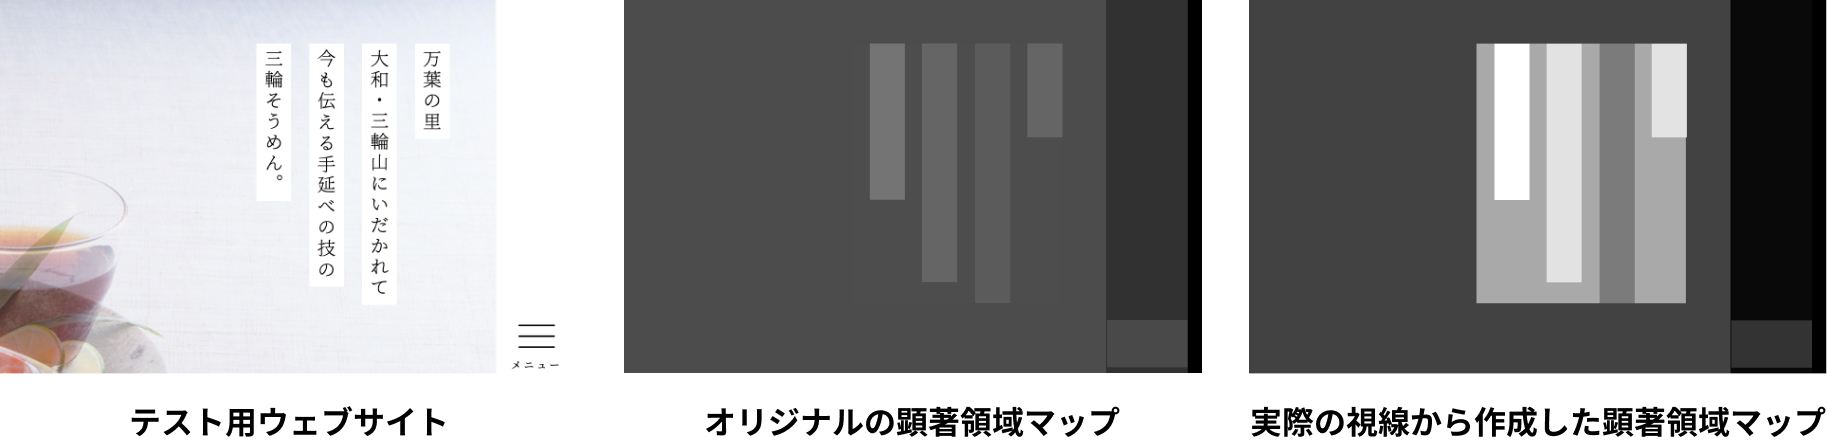
\includegraphics[width=12cm]{figures/06_textbias.jpg}
  \caption{テキスト箇所の顕著性評価比較}
  \label{fig_textbias}
\end{figure}

\par ウェブページには自然画像とは異なり様々なウェブページ固有の要素が存在する。その中の一つであるテキスト要素は自然画像にはほとんど存在せずあまり顕著度が高く評価されないがウェブページには多く存在する。図\ref{fig_textbias}にウェブページのテキスト表示箇所のオリジナルモデルの顕著領域マップと実際の視線データから作成した顕著領域マップの比較を示す。図から分かる通り人はテキスト要素に注目する傾向が高いが、Itti-Kochらのモデルなどの自然画像向け顕著性マップ生成モデルはテキストの顕著度をあまり高く評価しない。テキスト要素の顕著度を正しく評価するために該当要素の顕著度を高くするように重み付けを行った。


\subsubsection{要素の位置による重み付け}\label{subsec:system03-2}
\par 関連研究でも触れたShenらの人間の目の視線を測定するアイトラッカーを用いてウェブページの顕著性を測定した実験によると、図\ref{fig_shen-experience}に示すようにテキスト中心と画像中心とテキスト画像が混合した全てのウェブページにおいて人は左上の領域と中心付近に目線が行く傾向が判明した。ウェブページの左上から中央にかけての領域に注目が集まるの現象はf-biasと言う名で一般的に知られており、本システムでも左上の領域と中心付近で顕著度が高くなるように重み付けを行う。


\par 本システムの位置情報による重み付けの手法をアルゴリズム\ref{alg:weight-position}に示す。要素の中心点の位置によって要素の顕著度の重み付けを行うことにした。左上の領域に大きな重みをつけるtop-left biasについては、横軸方向にどれだけの重みの差をつけるかを表すplace\_weight\_xと縦軸方向にどれだけの重みの差をつけるかを表すplace\_weight\_yの2つの数値を与える事で表現した。また、中心領域に大きな重みをつけるcenter biasにおいては中心部と最外部でどれだけ重みの差をつけるかを表すplace\_weight\_cを与える事で表現した。さらにtop-left biasとcenter biasを組み合わせる事で左上と中央部分に大きな重みをつけるf-biasを表現する。本研究においては横軸の重みの差を表すplace\_weight\_x = 0.1に縦軸の重みの差を表すplace\_weight\_y = 0.4に中心の重みの差を表すplace\_weight\_c = 0.2に設定した。正方形の20$\times$20マスのブロックをウェブページに見立てて重みの数値をシミュレーションした結果を図\ref{fig_fbias}に示す。左図はtop-left biasを、中央はcenter biasを、右図は2つを組み合わせたf-biasを表す。また、赤色に近くほど重みの数値が大きく白色に近くほど数値が小さいことを表す。さらに、図\ref{fig_fbias-test}にテスト用の同じ色の正方形を等間隔で並べたウェブページを入力した時の結果を示す。重み付け前の顕著性マップでは全ての正方形が同じ明度で表わされているが、重み付け後の顕著性マップでは左上から中央にかけての正方形の明度が高く表わされている事が確認できる。なお、認識しやすいように重み付け後の顕著性マップには顕著度のランキングを緑色の枠線の色で表している。

\par 最後に、要素毎に以上の重み付け処理を行なった結果の顕著度を最終的な出力に使用する為にCSVファイルに追記する。

\begin{algorithm}[H]
    \caption{位置情報による重み付け(F-bias)}
    \label{alg:weight-position}
    \begin{algorithmic}
    \Function{calc\_salient\_level}{start\_x, start\_y, size\_w, size\_h}
    \State salient\_level $ \leftarrow $ 要素の明度の平均値(0-255)
    \State width $ \leftarrow $ 顕著性マップの幅(px)
    \State height $ \leftarrow $ 顕著性マップの高さ(px) 
    \State place\_weight\_x $ \leftarrow $ 0.1 //横軸方向の重み
    \State place\_weight\_y $ \leftarrow $ 0.4 //縦軸方向の重み
    \State place\_weight\_c $ \leftarrow $ 0.2 //中心方向の重み
    \If{$size\_w < width$ and $size\_h < height$}
        \State x\_bias $ \leftarrow $ 1-(place\_weight\_x-((width-(start\_x+$\frac{size\_w}{2}$))*$\frac{place\_weight\_x}{width}$))
        \State y\_bias $ \leftarrow $ 1-(place\_weight\_y-((height-(start\_y+$\frac{size\_h}{2}$))*$\frac{place\_weight\_y}{height}$))
        \State top\_left\_bias $ \leftarrow $ x\_bias * y\_bias
        \State center\_bias\_x $ \leftarrow $ $|\frac{width}{2}-(start\_x+\frac{size\_w}{2})|^2$
        \State center\_bias\_y $ \leftarrow $ $|\frac{height}{2}-(start\_y+\frac{size\_h}{2})|^2$
        \State center\_bias $ \leftarrow $ $\sqrt{center\_bias\_x + center\_bias\_y} $
        \State salient\_level $ \leftarrow $ salient\_level*(topleft\_bias - (place\_weight\_c * center\_bias))
    \EndIf
    \State \Return salient\_level
    \EndFunction
    \end{algorithmic}
\end{algorithm}

\begin{figure}[H]
    \centering
    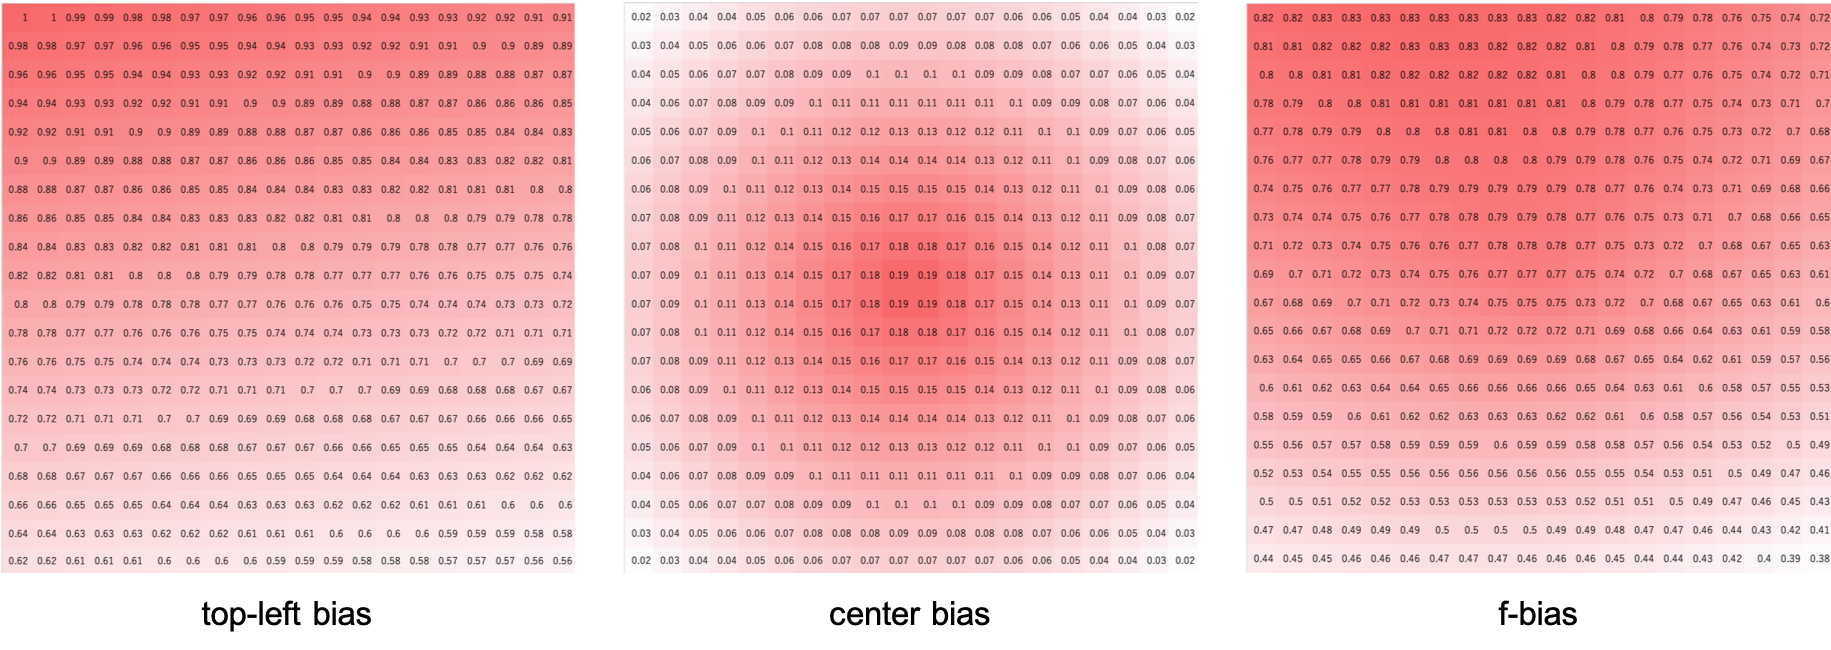
\includegraphics[width=12cm]{figures/fbias.png}
    \caption{位置情報による重み付けのシミュレーション}
    \label{fig_fbias}
\end{figure}

\begin{figure}[H]
    \centering
    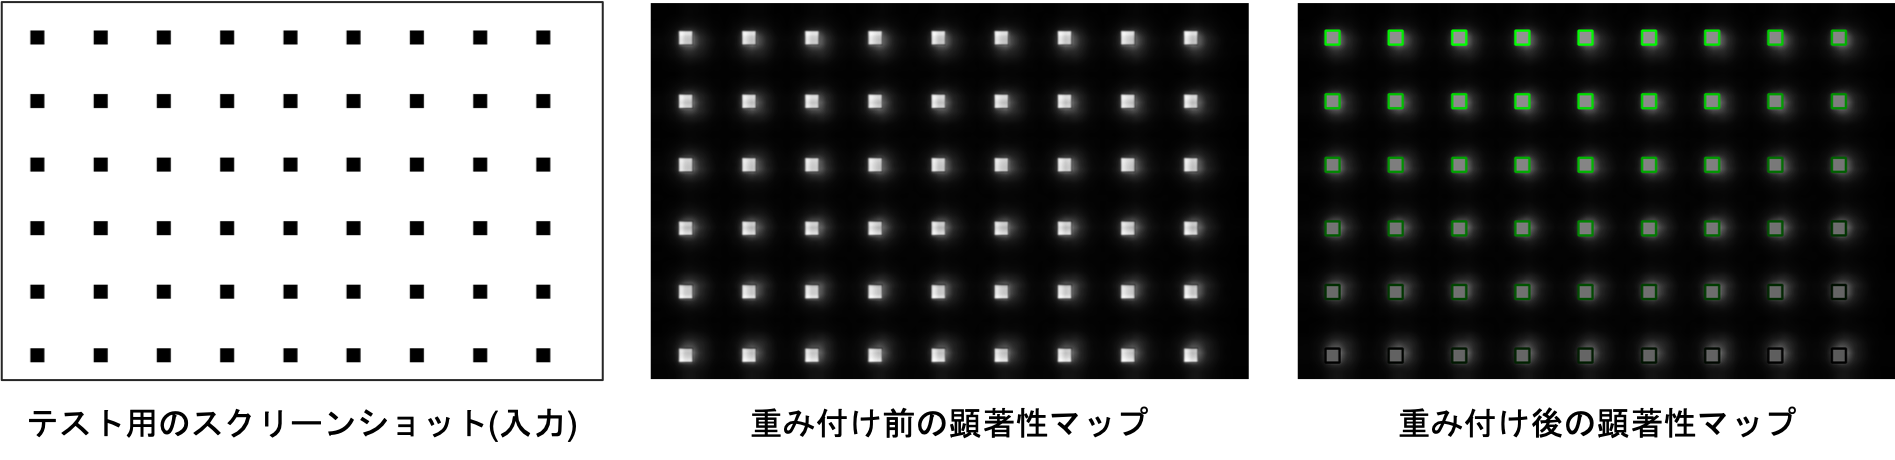
\includegraphics[width=12cm]{figures/fbias-test.png}
    \caption{テスト用ページを入力して得た顕著性マップ}
    \label{fig_fbias-test}
\end{figure}


\subsection{顕著領域の視覚化}\label{subsec:system04}
% 領域を塗りつぶして生成する顕著性マップと重要領域のランキングの生成方法の記述
\par ここでは第\ref{subsec:system03}節で計算した顕著度を元に顕著領域の視覚化を行う。本システムでは、顕著度が高い重要領域を要素単位で塗りつぶした顕著領域マップと特に顕著度が高い要素を一つにまとめた集約図の2つの出力を行う。顕著領域の視覚化の流れを図\ref{fig_system04}に示す。

\begin{figure}[H]
    \centering
    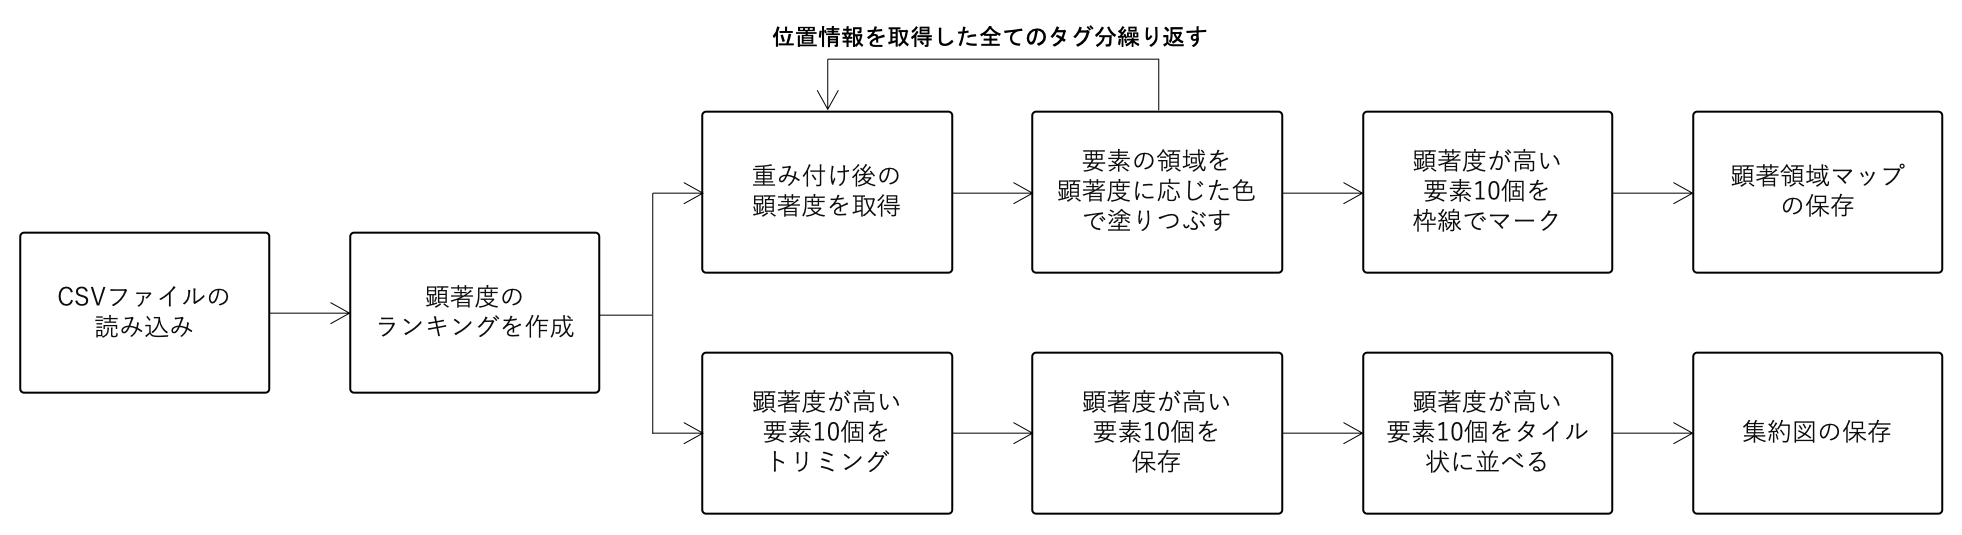
\includegraphics[width=12cm]{figures/system04.png}
    \caption{顕著領域の視覚化の流れ}
    \label{fig_system04}
\end{figure}

\subsubsection{顕著度ランキングの生成}\label{subsec:system04-1}
\par 顕著領域マップと集約図の生成にあたり、第\ref{subsec:system03}節で計算した顕著度のランキングを作成する。顕著度ランキングの計算アルゴリズムをアルゴリズム\ref{alg:lanking}に示す。まず始めに、第\ref{subsec:system03}節でCSVに保存した顕著度を顕著度が高い順にソートする。本来であれば、顕著度が高い順にランキングを付ければ良いが、図\ref{fig_system4-rank}に示すように同一要素を内包している他の要素も顕著度が高く評価されてしまう問題が生じる。同じ要素が顕著度ランキングに何度も出現する事は問題である為、一度顕著度が高いと評価した要素を内包する外部の要素をNGリストに格納して顕著度ランキングに入らないように評価する。



\newpage
\begin{algorithm}[H]
    \caption{顕著度ランキング}
    \label{alg:lanking}
    \begin{algorithmic}

    \State stag\_list $ \leftarrow $ CSVの読み組み, tag\_list\_num $ \leftarrow $ CSVの行数
    \State salient\_level = [] // 顕著度を格納するリスト, ng\_list = [] // NGリスト
    \State high\_element\_list = [] // 顕著度ランキングを格納するリスト
    \For{$i$ in $range(tag\_list\_num)$}
        \State salient\_level.append(tag\_listのi行目の要素の顕著度)
    \EndFor    
    \State salient\_level\_sort $ \leftarrow $ salient\_levelをソート
    \State salient\_num $ \leftarrow $ 10, temporal\_num $ \leftarrow $ 1, salient\_num\_first $ \leftarrow $ salient\_num

    \While{while salient\_num $>$ 0}
        \State most\_salient $ \leftarrow $ salient\_level\_sort[tag\_list\_num - temporal\_num]
        \If{(most\_salient in ng\_list) == False}
        \State start\_x, start\_y, end\_x, end\_y $\leftarrow$ CSVのmost\_salient行目から取得
        \State size $\leftarrow$ CSVからmost\_salient行目の要素のwidth $*$ heightを取得
        \If{(end\_x $-$ start\_x)/(end\_y $-$ start\_y) $<$ 10}
        \State high\_element\_list.append(most\_salient)
        \State salient\_num $\leftarrow$ salient\_num - 1
        \For{$i=1$ in $range(tag\_list\_num)$}
        \If{(most\_salient in ng\_list) == False}
        \State r\_start\_x, r\_start\_y, r\_end\_x, r\_end\_y $\leftarrow$ i行目から取得
        \State r\_size $\leftarrow$ CSVからi行目の要素のwidth*heightを取得
        \If{i行目要素とmost\_salient行目要素が内包関係}
        \If{r\_size $-$ size $<$ 200 $or$ size $-$ r\_size $<$ 200}
        \State ng\_list.append(i) //NGリストにi行目要素を格納
        \EndIf
        \EndIf
        \EndIf
        \EndFor 
        \EndIf
        \Else
        \State temporal\_num $\leftarrow$ temporal\_num $+$ 1
        \EndIf
    \EndWhile
    \end{algorithmic}
\end{algorithm}

\begin{figure}[H]
    \centering
    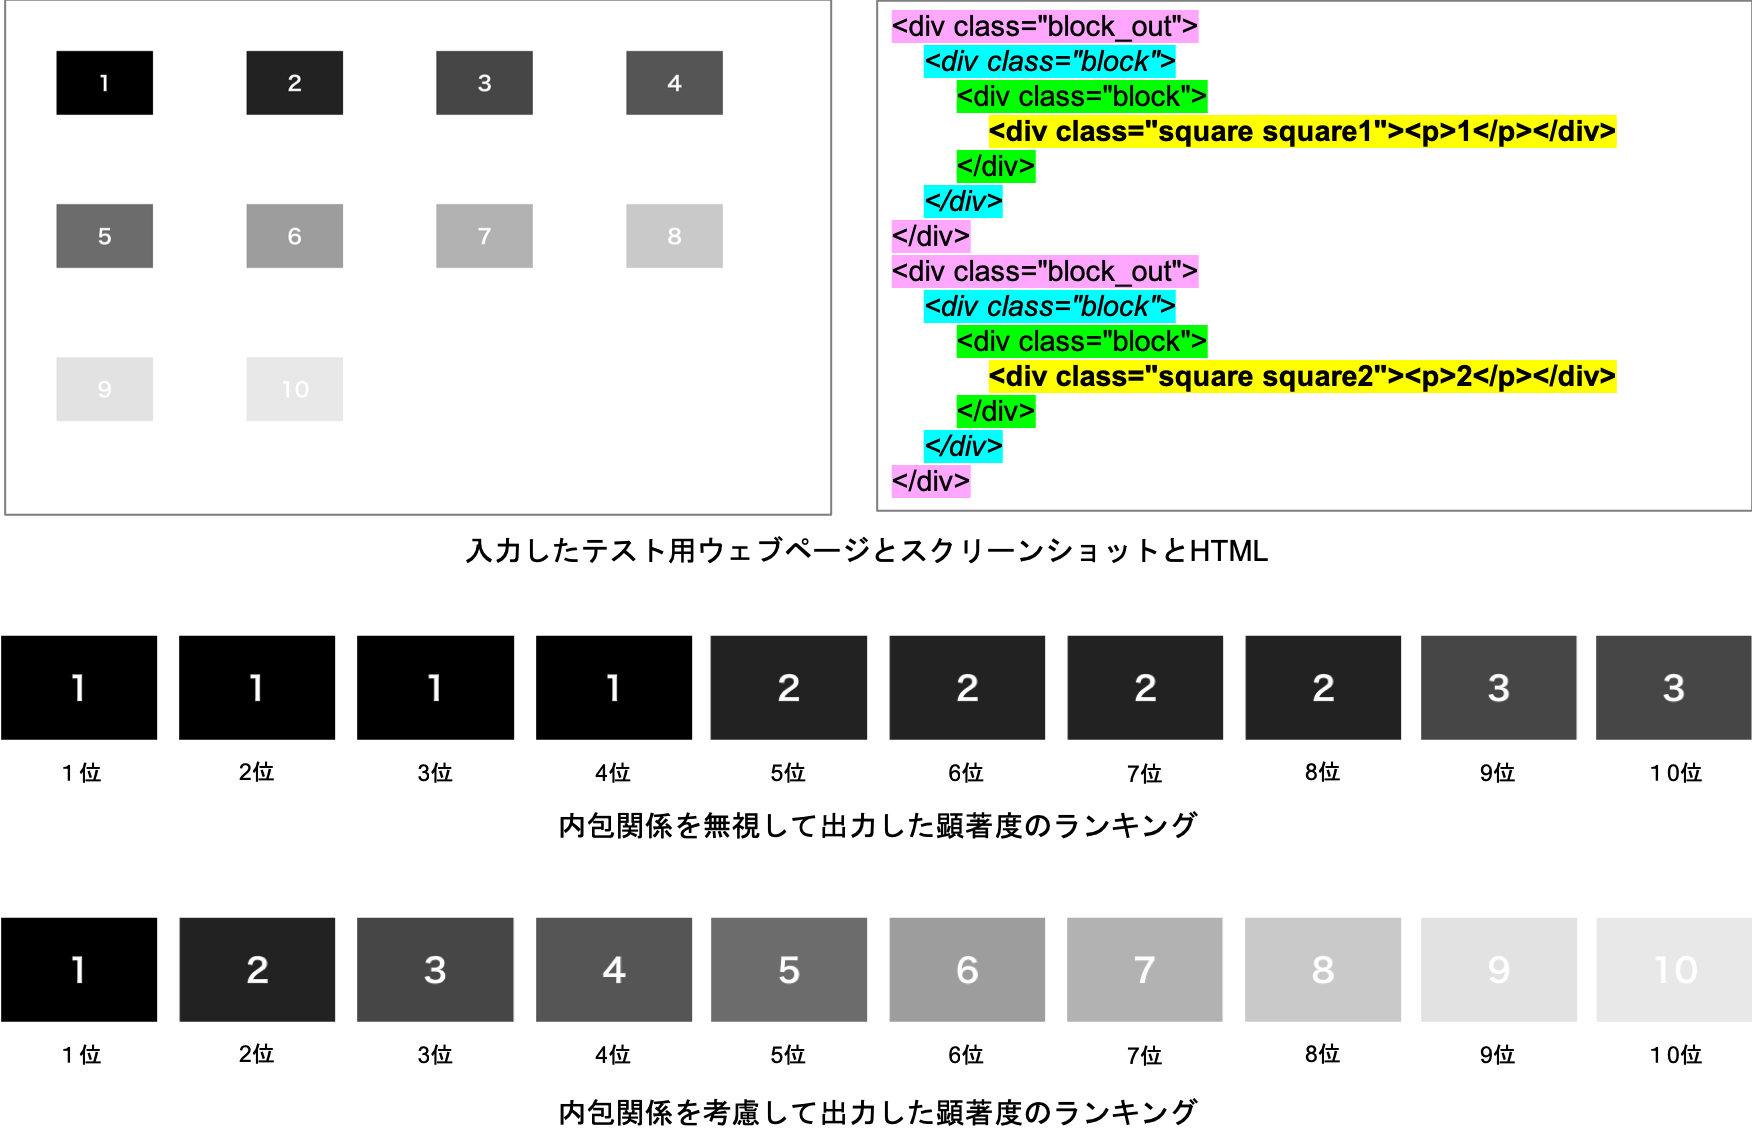
\includegraphics[width=12cm]{figures/include-rank.png}
    \caption{要素の内包関係を考慮した時としない時の顕著度ランキング}
    \label{fig_system4-rank}
\end{figure}

\subsubsection{顕著領域マップの生成}\label{subsec:system04-1}
\par 顕著領域マップの生成方法について説明する。第\ref{subsec:system03}節で計算した顕著度は0$\sim$255の範囲内の実数で表わされている。位置情報を取得した画面上に表示されている全ての要素の領域をこの顕著度を明度とした長方形で塗り潰す。また、第\ref{subsec:system03-1}節で説明した重み付けにより全体的に顕著度が低くなっている為、補正値を与える事ですべての要素の顕著度を補正値分高くすることとする。
\par さらに、特に顕著度が高い重要領域を視覚化する為に第\ref{subsec:system04-1}項で作成した顕著度ランキングの上位10個の要素の外枠を顕著度が高い順に明るい緑色の線で描写する。以上の作業を行う事で顕著領域マップの生成を行う。図\ref{fig_tile-example}に第\ref{subsec:system04-1}項で説明したテスト用ウェブページのURLを入力して生成された顕著領域マップの例を示す。

\subsubsection{集約図の生成}\label{subsec:system04-2}
\par 集約図の生成方法について説明する。第\ref{subsec:system04-1}項で作成した顕著度ランキングを元に顕著度が上位10個の要素の領域をスクリーンショットから切り取りタイル状に並べる。本システムでは上段に上位2個を、中段に3位$\sim$5位の3個を、下段には6位$\sim$10位の5個を並べる事で表現した。図\ref{fig_tile-example}に第\ref{subsec:system04-1}項で説明したテスト用ウェブページのURLを入力して生成された集約図の例を示す。


\begin{figure}[H]
    \centering
    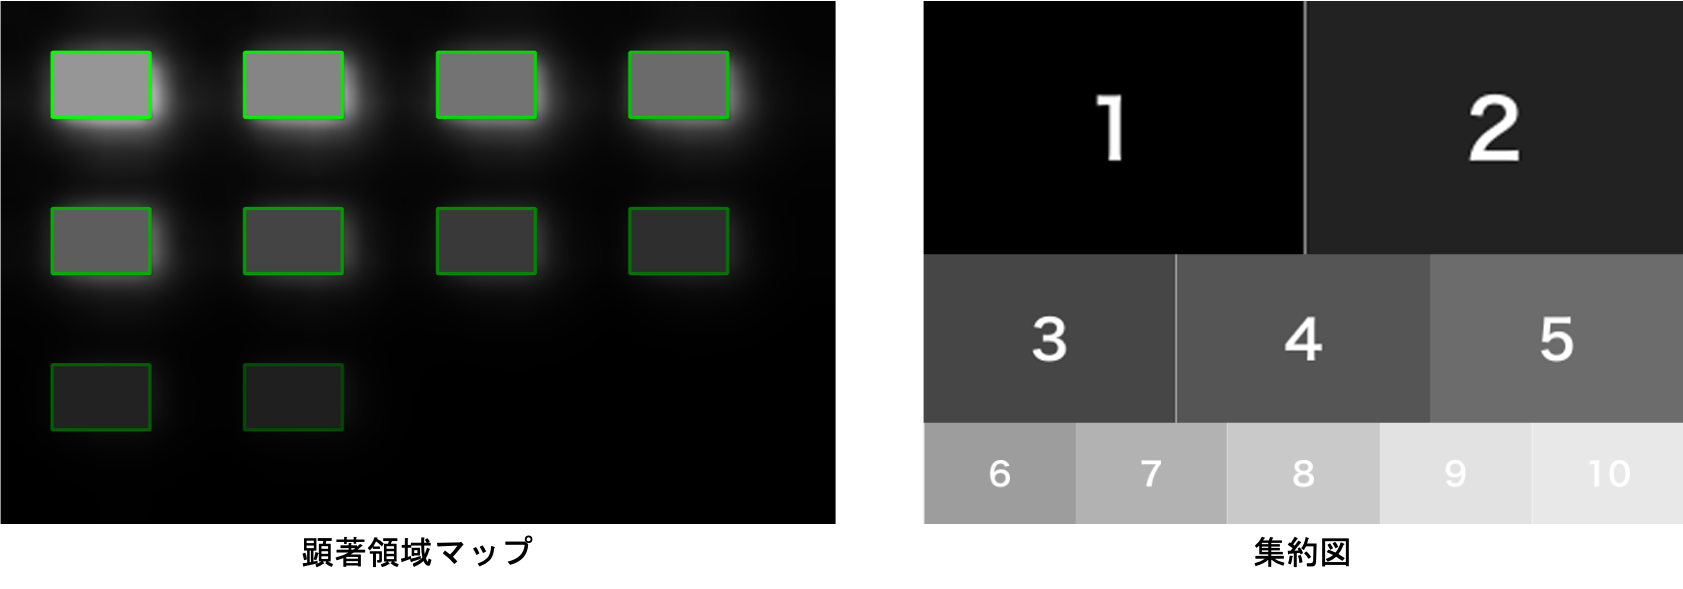
\includegraphics[width=10cm]{figures/example-output.png}
    \caption{生成される顕著領域マップと集約図の例}
    \label{fig_tile-example}
\end{figure}
